\subsection{Examples}

\begin{frame}[fragile]
	\begin{figure}
		\centering
		\begin{tikzpicture}[ scale = 0.6 ]
	\tikzset{ vertex/.style = { shape = rectangle , draw , minimum size = 2em , rounded corners } }
	\tikzset{ edge/.style = { ->,> = latex' } }
	% vertices
	\node[ vertex ] (B) at  ( 4 , 4 ) { ${Buying}$ } ;
	\node[ vertex ] (D) at  ( 2 , 2 ) { ${Doors}$ } ;
	\node[ vertex ] (P) at  ( 6 , 2 ) { ${Persons}$ } ;
	\node[ vertex ] (M) at  ( 0 , 0 ) { ${Mantain}$ } ;
	\node[ vertex ] (S) at  ( 4 , 0 ) { ${Safety}$ } ;
	\node[ vertex ] (L) at  ( 8 , 0 ) { ${Luggage}$ } ;

	%edges
	\draw[ edge ] (B) to (D) ;
	\draw[ edge ] (B) to (P) ;
	\draw[ edge ] (D) to (M) ;
	\draw[ edge ] (D) to (S) ;
	\draw[ edge ] (P) to (S) ;
	\draw[ edge ] (P) to (L) ;
\end{tikzpicture}
	\end{figure}
	\begin{block}{}
		$\P( B , M , D , P , L , S ) = \P( B ) \P( D \mid B ) \P( P \mid B ) \P( M \mid D ) \P( S \mid D , P ) \P( L \mid P )$
	\end{block}
	This requires $4 + (4 \times 4) + (3 \times 4) + (4 \times 4) + (3 \times 4 \times 3) + (3 \times 3) = 93$ probabilities instead of $1728$
\end{frame}
	
\begin{frame}[fragile]
	\begin{columns}
		\begin{column}{.3\linewidth}
			Consider each variable has $k$ values:\\
			We requires $k^{33}$ probabilities without independences.
		\end{column}
		\begin{column}{.6\linewidth}
			\begin{figure}
				\centering
				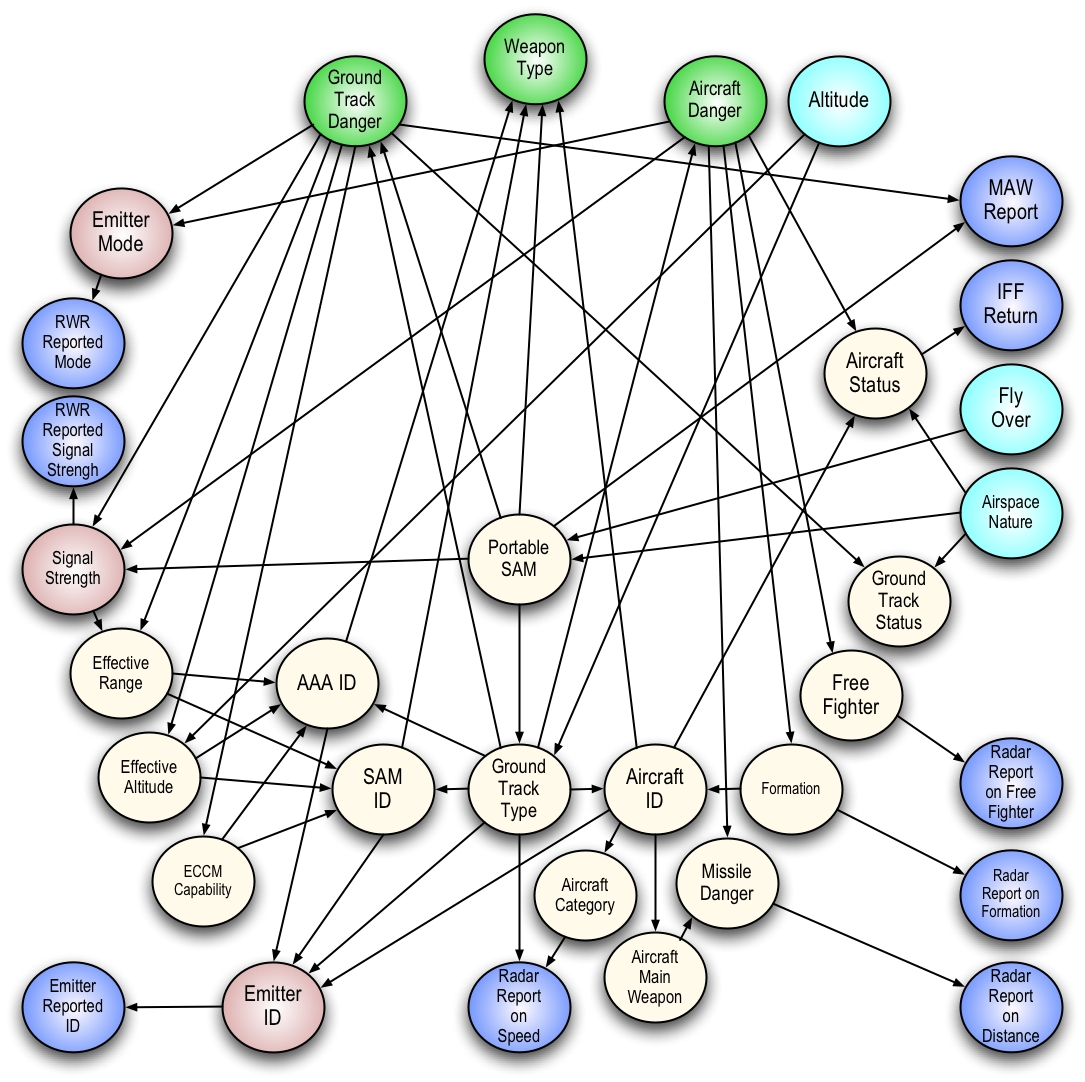
\includegraphics[height=17em]{images/complexbn}
			\end{figure}
		\end{column}
	\end{columns}
\end{frame}